\documentclass[border=15pt, multi, tikz]{standalone}
\usepackage{tikz}
\usetikzlibrary{shapes,arrows,positioning}

% Define colors
\definecolor{ConvColor}{rgb}{0.9,0.8,0.5} % Yellowish
\definecolor{ConvReluColor}{rgb}{1,0.6,0} % Orange
\definecolor{LinearColor}{rgb}{0,0,1} % Blue
\definecolor{OutputColor}{rgb}{0,1,0} % Green

% Define styles
\tikzset{
    box/.style={rectangle, draw, minimum width=2cm, minimum height=1cm, text centered},
    conv/.style={box, fill=ConvColor},
    linear/.style={box, fill=LinearColor},
    output/.style={box, fill=OutputColor},
    connection/.style={-latex, thick}
}

\begin{document}

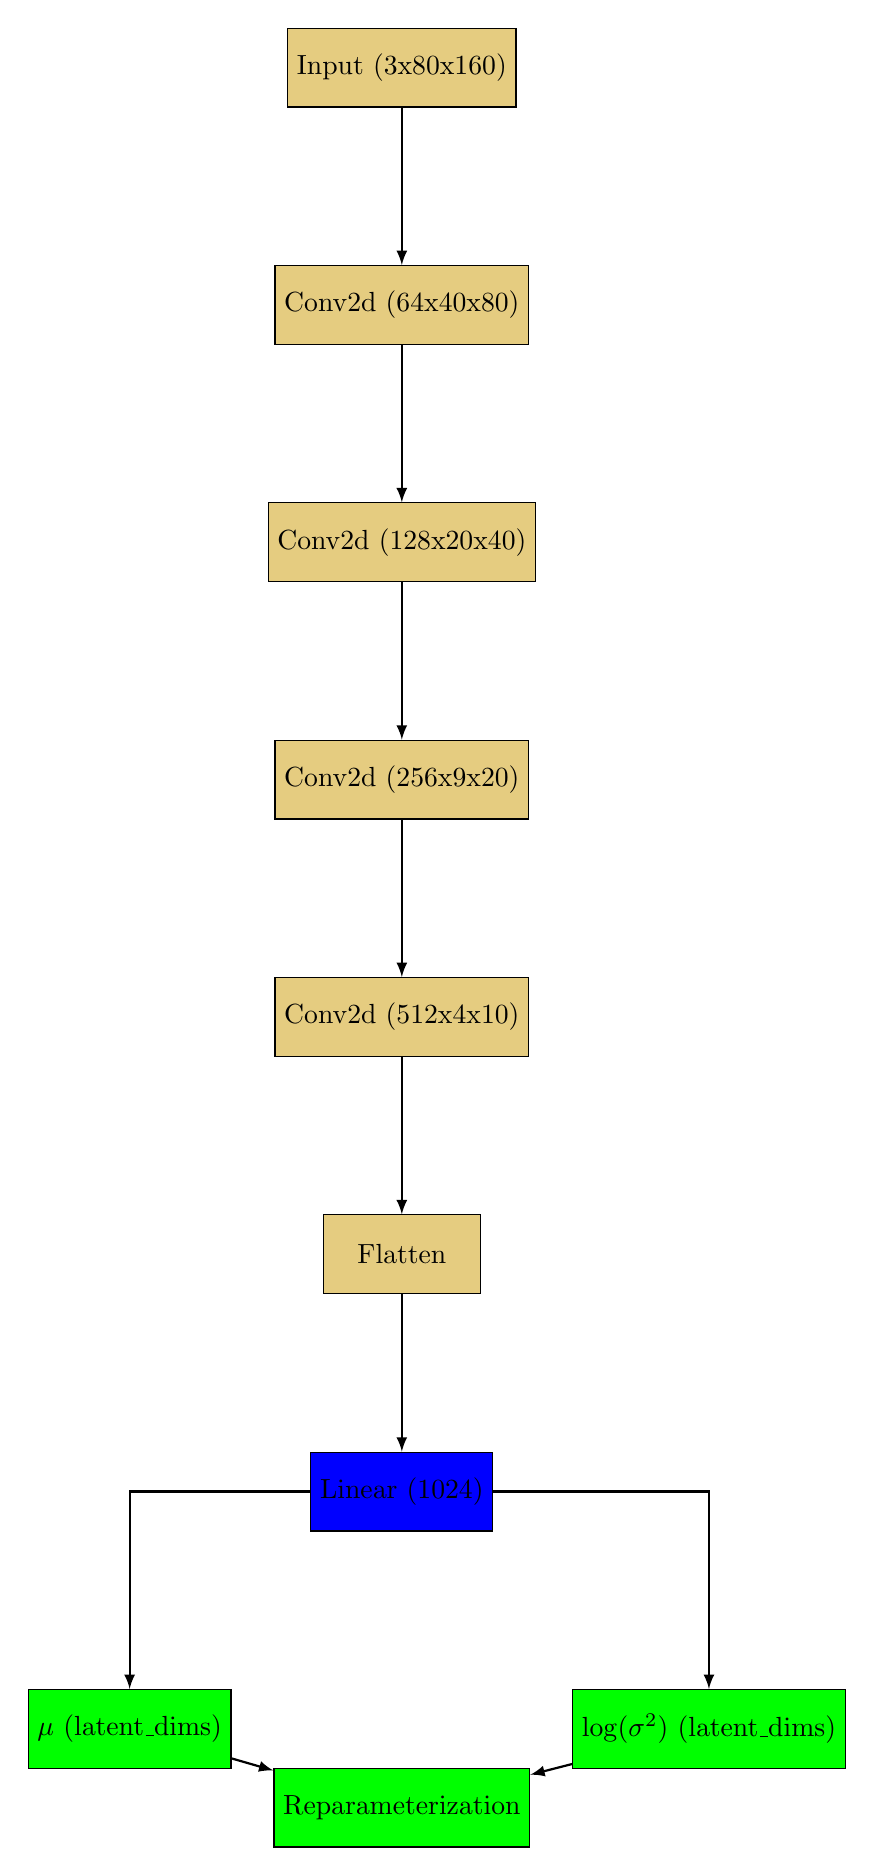
\begin{tikzpicture}[node distance=2cm and 1cm]

% Input layer
\node (input) [conv] {Input (3x80x160)};

% Encoder layers
\node (conv1) [conv, below=of input] {Conv2d (64x40x80)};
\node (conv2) [conv, below=of conv1] {Conv2d (128x20x40)};
\node (conv3) [conv, below=of conv2] {Conv2d (256x9x20)};
\node (conv4) [conv, below=of conv3] {Conv2d (512x4x10)};

% Flatten layer
\node (flatten) [conv, below=of conv4] {Flatten};

% Linear layer
\node (linear) [linear, below=of flatten] {Linear (1024)};

% Mu and Logvar layers
\node (mu) [output, below left=of linear] {$\mu$ (latent\_dims)};
\node (logvar) [output, below right=of linear] {$\log(\sigma^2)$ (latent\_dims)};

% Reparameterization trick
\node (reparam) [output, below=of linear, yshift=-1cm] {Reparameterization};

% Connections
\draw [connection] (input) -- (conv1);
\draw [connection] (conv1) -- (conv2);
\draw [connection] (conv2) -- (conv3);
\draw [connection] (conv3) -- (conv4);
\draw [connection] (conv4) -- (flatten);
\draw [connection] (flatten) -- (linear);
\draw [connection] (linear) -| (mu);
\draw [connection] (linear) -| (logvar);
\draw [connection] (mu) -- (reparam);
\draw [connection] (logvar) -- (reparam);

\end{tikzpicture}

\end{document}